\documentclass{article}

% Symbols
\usepackage{amsfonts, amsthm}
\usepackage{upgreek}
\usepackage{physics}
\usepackage{cancel}
\usepackage{amssymb, latexsym, amsmath}
\usepackage{import}

%Algorithms
\usepackage[ruled,lined,linesnumbered,commentsnumbered]{algorithm2e}

%% Identación
\setlength{\parindent}{0cm}

% Código
\newcommand{\code}[1]{\textcolor{white!25!black}{\texttt{#1}}}
\usepackage{listings}

%AMS
\usepackage{amsthm}
\newtheorem{algo-thm}{Algoritmo}

% Graphics
\usepackage{graphicx}
\usepackage{pgf}

% Margins
\addtolength{\voffset}{-1.5cm}
\addtolength{\hoffset}{-1.5cm}
\addtolength{\textwidth}{3cm}
\addtolength{\textheight}{3cm}

%Header-Footer
\usepackage{fancyhdr}
\renewcommand{\headrulewidth}{1pt}

\newcommand{\set}[1]{
  \left\{ #1 \right\}
}

\footskip = 50pt
\renewcommand{\headrulewidth}{1pt}

\pagestyle{fancyplain}

\begin{document}
	\title{UNIVERSIDAD NACIONAL AUT\'ONOMA DE M\'EXICO\\ Facultad de Ciencias}
\author{Integrantes:\\
  Diego Angel Rosas Franco\\
  Adri\'an Aguilera Moreno\\
  Marco Antonio Rivera Silva}
\date{}
\maketitle
\begin{center}
  
\includegraphics[scale=0.20]{../Portada/Portada}\\[0.4cm]
  \Large
  \bf{Modelado y programación}
  \normalsize
\end{center}
\newpage
\fancyhead[r]{ Modelado y programación 2022-2}


	\section*{\LARGE{Práctica 2}}

Menciona los principios de diseño esenciales del patrón State, Template e Iterator:

\subsubsection*{Template}
Principios de diseño esenciales:
\newcommand{\localtextbulletone}{\textcolor{black}{\raisebox{.45ex}{\rule{.6ex}{.6ex}}}}
\renewcommand{\labelitemi}{\localtextbulletone}
\begin{itemize}
\item \textbf{Template define los pasos de un algoritmo en un método (un esqueleto):}
  
  En Java, dentro de este método tenemos otros métodos que estarían representando los
  pasos del algoritmo.
\item \textbf{Template define algunos pasos de este algoritmo y otros los deja a
  criterio de las subclases que implementan este algoritmo:}
  
  En Java, podemos ver a estos pasos como métodos ya definidos y que las subclases no
  necesitarán volver a definir, y métodos abstractos, que son aquellos pasos que deben
  definir las subclases según les corresponda.

\item \textbf{Algunos de estos pasos (métodos) ya definidos pueden ser hooks:}
  
  Es decir, las subclases deben decidir si la implementación que tienen coincide
  con su fin o deben redefinirla.
  
\item Evita que subclases reescriban código (pasos) de un determinado algoritmo.
\item Permite a las subclases adaptar el algoritmo sin modificar la estructura del mismo.
\end{itemize}

Desventajas:
\begin{itemize}
  \item \textbf{Agregar un paso implicaría tener que implementar ese paso (si se requiere) en todas las subclases.}
  Es decir, si en nuestro algoritmo agregamos uno o más pasos extras que las subclases deben implementar, este cambio puede ser muy exhaustivo si es que se tienen demasiadas subclases.

\item \textbf{Si se usa mal el patrón perderíamos flexibilidad en el código.}
  
  Ya que al tener una estructura definida, y querer un cambio radical en el algoritmo,
  tendríamos que implementar uno nuevo.  
\end{itemize}

\subsubsection*{State}
Principios de diseño esenciales:
\begin{itemize}
\item Permite a un objeto cambiar su comportamiento (indistintamente) de manera instantánea
  en tiempo de ejecución, y el objeto cambia cuando su estado interno se ve modificado de
  alguna manera.
\item El patrón de diseño “state” se usa cuando una clase (una entidad) tiene distintas fases
  (estados) y en cada una de estas su comportamiento es distinto.
\item Se encapsulan las acciones a realizar dando como resultado un estado.
\end{itemize}

Desventajas:
\begin{itemize}
\item Si se tienen demasiados estados y hay varias conexiones entre ellos, puede
  resultar difícil el saber como se relacionan teniendo solamente el código.
\item El impacto en espacio, ya que por cada estado tendríamos una clase y si son
  demasiados estados, sería mucho espacio.
\end{itemize}

\subsubsection*{Iterator}
Principios de diseño esenciales:
\begin{itemize}
\item Nos permite acceder a los elementos de un objeto que los contiene de manera
  secuencial sin exponer su representación interna mediante Iteradores.
\item Ayuda a generalizar la tarea de recorrer los elementos de una estructura con un Iterador.
\end{itemize}

Desventajas:
\begin{itemize}
\item \textbf{El iterador afecta el dinamismo de la estructura:}
  
  Por ejemplo, podría surgir un cambio en la estructura, ya sea la inserción
  o eliminación de un elemento, causando que el Iterador tenga que actualizarse
  y posicionarse donde se había quedado o en una determinada posición.
\end{itemize}

\subsection*{Instrucciones de instalación, compilación y ejecución.}
Se dará por hecho que el usuario sabe moverse en terminal.\\

\subsubsection*{Requerimientos previos:}
\begin{itemize}
\item[-] Se debe contar con Java en su computadora. De preferencia la versión más reciente.
\end{itemize}

\subsubsection*{Ejecución del proyecto:}
\begin{itemize}
\item[-] Si está leyendo esto significa que desempaquetó con éxito el proyecto.
\item[-] Abra su terminal y diríjase a la ruta donde desempaquetó el proyecto.
\item[-] Una vez estando en la ruta \code{Practica02\_NullPointerException}, diríjase a

  \code{Practica02\_NullPointerException/src/fciencias/modelado/}
\item[-] Ejecute: “javac Practica02.java”, esto generará los .class del proyecto.
\item[-] Ejecute: “java Practica02”, esto ejecutará el proyecto mostrándole el menú solicitado para la practica.
\end{itemize}

\subsection*{Diagrama UML:}
\begin{center}
  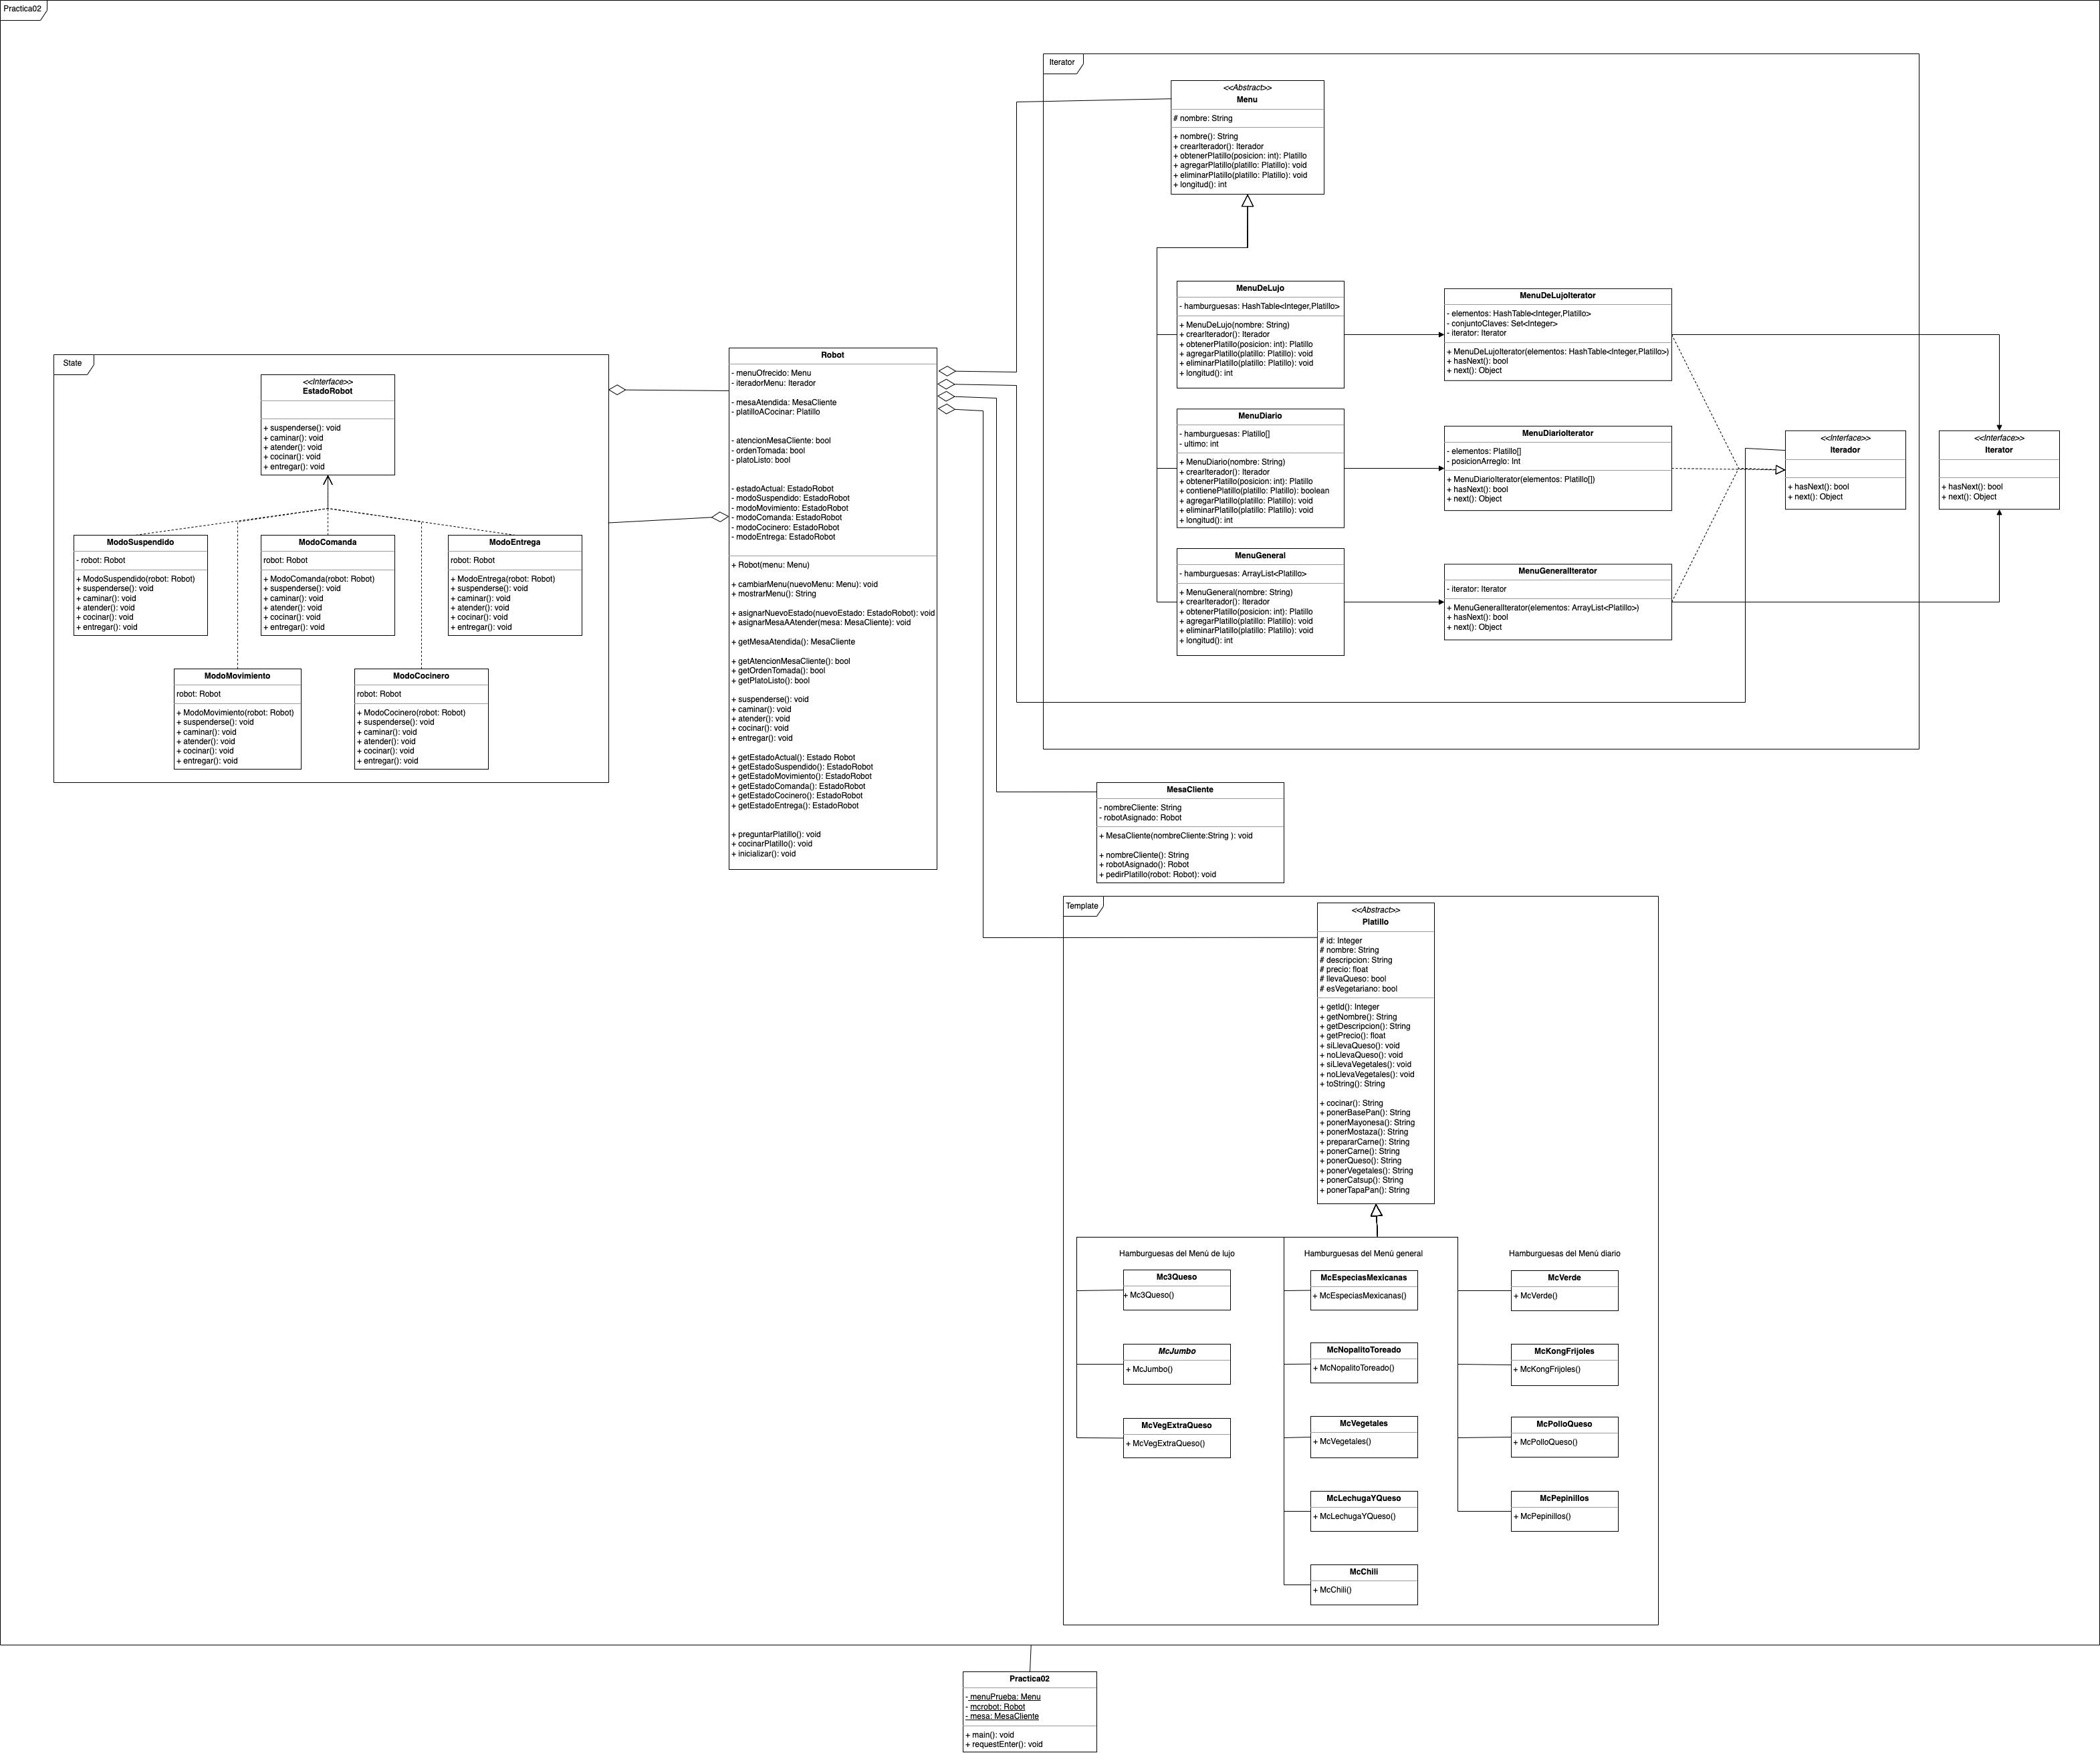
\includegraphics[scale=0.12]{./Practica02UML.png}
\end{center}

\subsection*{Diagrama de Estados:}
\begin{center}
  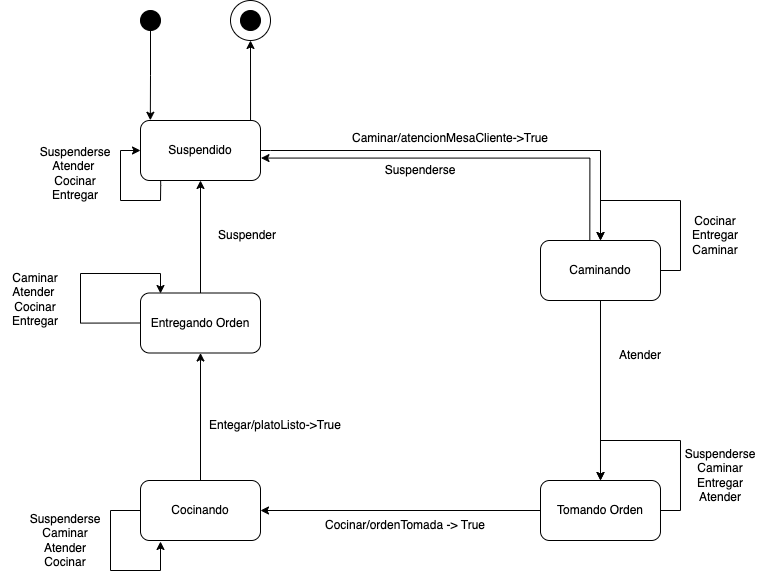
\includegraphics[scale=0.40]{./Practica02DiagramaDeEstados.png}
\end{center}


\end{document}
